\section{Designing FSO Links for Flexible Inter-Rack Networking}
\label{sec:fso}

\blue{Our goal in this section is to present the design of FSO transceiver modules
that have the needed properties for the design of a flexible inter-rack
fabric, i.e., (i) size, power and cost effectiveness, (ii) ability to provide
10-100Gbps data rate, (iii) ability to align with the needed precision, (iv)
ability to steer precisely and with low latency.} \samir{These concepts 
should ideally come up earlier in section 2.3. We are anyway saying something 
like this there already.}


In a datacenter, the space above the racks is a natural choice for laser
propagation as this space is roughly free from obstruction.  The FSO
transceivers thus will be anchored on
the top of the rack and connected to ToR switch ports. The transceivers themselves
will either be staggered so that they themselves do not present obstructions
or mirrors in the ceiling (and possibly additional mirrors on the beam path for
redirection) will be used to avoid obstructions. (More on this momentarily.) \blue{Overall, 
a design goal is that a single FSO transceiver assembly including  necessary alignment
and beam redirection
machinery can be put together within roughly about 3"x8" footprint such as that a few
tens of such devices can be packed on the top of a rack.} Additionally, the 
power consumption should be modest, not exceeding that of the electrical switched
networks they are replacing. Further, they must be cost-competitive to such
networks as well. 

%A critical task in
%the project will be designing the op-tical elements (e.g., mirrors, lenses) and
%their precise positioning such that they operate for wide range of distances,
%e.g., few meters for neighboring racks or over 100m for distant racks in a
%large data center.

The broad design goals above do not lend themselves to using 
commodity FSO transceivers directly. 
The use case for these
devices is terrestrial long distance (miles) communication~\cite{}.\footnote{FSOs
are also used in satellite and space communications. But FSOs used
there are certainly not commodity.}
Their design cannot optimize on size, power or
cost.\footnote{A typical commercially available system~\cite{lightpointe} 
is roughly 2 cubic feet, costs \$5-10K for a
single link, consumes XXX watts.} The reason for this is that they have to
overcome several outdoor challenges in laser propagation (e.g., beam path
variations due to scattering from fog or dust and due to significant
temperature/humidity variations along long paths, larger transmit power
requirements to account for path loss as well as divergences over long
distances, non-trivial alignment problems due to structural swaying etc). 
These challenges largely go away in datacenters thus opening up a pathway 
for size, power, and cost-optimized design. But the new requirement
of fast reconfiguration arises, where the FSO beam path must be redirected
at a fast time scale
between a set of possible receivers to enable a switching 
in the interconnection fabric. 
This necessitates a fundamentally new design of FSO communication 
for the emerging use case in datacenter. In the discussion that follows
we lay out the challenges and proposed approach in a two step 
process:
%
(i) Designing the basic  FSO link for a datacenter-scale operation, 
(ii) Fast beam redirection to enable reconfiguration.
Both must follow the required size, cost and power constraints. 



%. In addition, Firefly architecture will now 
%have thousands of FSO links with each rack carrying a few tens of FSO transceivers
%depending on the desired capacity. 
% 

%Size, cost and power now become central issues:
%Firefly will have thousands of FSO links and real estate on the top of the rack
%for deploying the transceivers are limited. Further, the design must be cost
%effective and power efficient  --- an argument put forward in
%Section~\ref{sec:mot}.  
%\vyas{this para can be shrunk .. there is some redundancy here. how abt starting with the conventional -- new requirements } \samir{now shrunk}
%

%Due to these unique needs, we have proposed a ground up design. However, we need to still rely on commodity components as much as possible to make an entire end-to-end prototype feasible within the budget/timeline of the project (described in Section~\ref{sec:evalplan}).  
%While this prototype will be of small scale, the description below articulates a pathway for designing scalable systems. \vyas{this para could go} 

\subsection{Designing FSO Link for \ArchName}

%\vyas{what reliability .. hardware/asic?}

\begin{task}
Design the FSO link including transmitter, receiver and the optical beam path
for effective datacenter scale operation.
\end{task}
\smallskip
An FSO communication link consists of two basic components: i) a transmitter
(TX) that is a modulated laser source (typically infrared), ii) a receiver
(RX) that is a high-speed optical detector along with a de-modulator, iii) the
optical path. A major step in our design is that we propose to repurpose
optical small form-factor pluggable (SFP) transceivers~\cite{} for TX and RX
components. Optical SFPs are used to inter-face optical fibers with
(electrical) packet switches. The advantage of this approach is that we can
exploit the large commodity market of optical SFPs that already operate at 10+
Gbps. This keeps the cost low in relation to a first-principles design of TX
and RX. The optical SFPs are also very small in size (\blue{state size??}) and
already contain very reliable, field-tested TX and RX components. They are also
indeed low power (\blue{state power??}). 
Without going into any quantitative analysis, we claim that the SFPs cannot be 
any added power burden as datacenters often use optical fibers for inter-rack
connectivity\footnote{whenever the cable length exceeds the distance
copper cables can carry at the highest data rates~\cite{}} interfaced via optical SFPs. 
%In any case, datacenters often use
%them regardless of the network architecture, whenever optical fibers need to be
%used to support high data rates at distances that standard copper cables are
%unable to carry~\cite{}. Thus, there is no added power burden from our use of
%optical SFPs.  
%\vyas{last two sentences are breaking the flow}
%\samir{now check.}


%\vyas{flow between prev this para is awkward} 

\paragraph*{Optical Path Design} 
After we have decided on the TX and RX hardware, the next design challenge 
is the optical path. The optical SFP is designed to interface
directly to an optical fiber\footnote{Typically, a fiber pair for bidirectional
communications. Single fiber SFPs~\cite{} are also possible where the laser and
detector at each end point are interfaced to the same fiber with two directions
operating at two different wavelengths. As would be apparent later, use of
single fiber SFPs make our approach easier as only one optical path needs to be
designed per FSO transceiver.}  with the fiber confining the beam via a series
of internal reflections. Instead now the laser beam launches directly into
free space, diverging in a
cone as it propagates\footnote{Note that this is a fundamental optical property
and unrelated to the use of SFPs.} quickly losing power. This divergence is typically
arrested using a suitably designed collimating lens on the optical path near
the TX. This makes the laser beams roughly parallel, now diverging at a very
slow rate – in the order of milli-radians or less. Finally a similar lens near
the RX focuses the beam back onto the detector. From basic optics, an inverse
relationship exists between the diameter of the propagating laser beam at the
so called ‘beam waist’ (the narrowest part of the beam near) and the rate at
which it diverges beyond this point (divergence angle). 

The above presents a fundamental tradeoff  that must be optimized,
a challenge we will undertake.  
A larger beam waist is better to keep the divergence negligible
and also to make the alignment easier (described next). But it also requires
a larger lens (size issue). Smaller diameters on the other hand may
make the beam diverge too quickly for it to be strong enough at the extreme
distances within the datacenter (say, 100m). But again, the topology design (Section~\ref{sec:topology})
may be able to bypass the need for very long distance links. 
%Beam
%diameter also influences alignment challenges that we will describe now.
% \vyas{para loses flow toward end .. maybe say keywords like challenge, solution etc to help keep flow?} 

\paragraph*{Alignment} The optical detector at RX gathers energy proportional
to its size (\blue{in the order of XX for SFPs}). Ideally, we do not want the
beam to have a much larger diameter at the RX than the detector size lest only
a very small fraction of the power will be captured that may not be enough for
reliable detection. Thus, both very large diameter beam waist and large divergences
may be poor design choices. On the other hand, large diameter helps in alignment
as small shifts in the optical path will have negligible effect in the detector
so long as the total energy received at the detector is above the detection
threshold.  This helps recovering from rack vibrations, jarring effects due to
maintenance, optical path drifts due to air temperature variations, and other
similar issues. If the beam diameter itself is not sufficiently large to
account for the above, small positioning corrections of the TX and/or RX will
be needed. 

\red{We plan to use piezoelectric positioners or thermal heaters with a high-thermal-expansion material can provide these needed precision corrections at reasonable costs.} The feedback needed to these corrections can be obtained from the DOM (digital optical monitoring) support already present in the optical SFP standard and carried on the I2C bus via the connectors on the module. If corrections on the RX side are insufficient and the TX side needs to be adjusted as well, the RF-based control mechanism will be used (discussed in Section~\ref{sec:evalplan}).



%\vyas{this design overview probably  needs to come much earlier in the section?}





\subsection{Re-configurability via Beam Path Redirection}

%\vyas{i think i liked the way of talking abt macro/micro alignment and
%saying there are two types of alignment problems that high-level flow is 
% missing here}

\begin{task}
Develop fast and effective beam path redirection techniques to achieve 
reconfiguration in the interconnection fabric.
\end{task}
\smallskip
In Firefly the ToR switches are to be interconnected via the FSO links to
create an FSO-based inter-rack fabric. To achieve reconfigurability in this
fabric, the beam from the TX must fundamentally be able to connect to 
multiple possible RXs on top of a {\em subset} of other racks.  
The reason it is a subset and not the entire set of racks is simply due to 
technology difficulties that will be apparent soon. 
%
This fundamentally gives
rise to three different types of beam 'movements'  or 'adjustments' that we must accommodate:
\begin{packedenumerate}
\item {\em Pre-configuration:} -- This describes setting up the FSO system such 
that an TX can have a link to any RX from a chosen subset. Again, technology limitations
may not allow any arbitrary subset -- giving rise to interesting topology design problems
described in Section~\ref{sec:topology}. 
\item{\em Reconfiguration:} -- This describes ensuring a TX can have a link to a chosen
RX in the chosen subset above. This must be done at a fast time scale, \blue{
in the order of ms or less.}
\item{\em Alignment:}  -- This caters to minor adjustment necessary to cater 
to beam misalignments due to vibrations, etc as described previously. 
\end{packedenumerate}
\samir{Two things related to the above: First, we need to discuss the terms used. Second, 
we could move this to the beginning of this section. 
But somehow it needs some background. So, I am saying this here, even though alignment
has been already been described. Also, since the pre- and re-config issues are 
coming up repeatedly, may be we can claim space in sec 4 and elsewhere by 
consolidating them in one place, i.e., here.}

For ease of understanding, we will present reconfiguration first. 
We will achieve reconfiguration via beam redirection using
two independent mechanisms: i) switching using switchable mirror 
and ii) steering using Galvo mirrors. They both present
certain tradeoffs. The impact of such tradeoffs in the overall performance is
unclear without a careful evaluation. Such an evaluation will be part of
our work. We anticipate that we will pick one or a combination design in our
final prototype and in future research.  This will also influence
our on pre-configuration topology design in Section~\ref{sec:topology}.  
%\vyas{maybe throw in a tie-in to 
% the section 4 algorithm on how to combine}

\begin{figure}[t]
\centering
\begin{tabular}{cc}
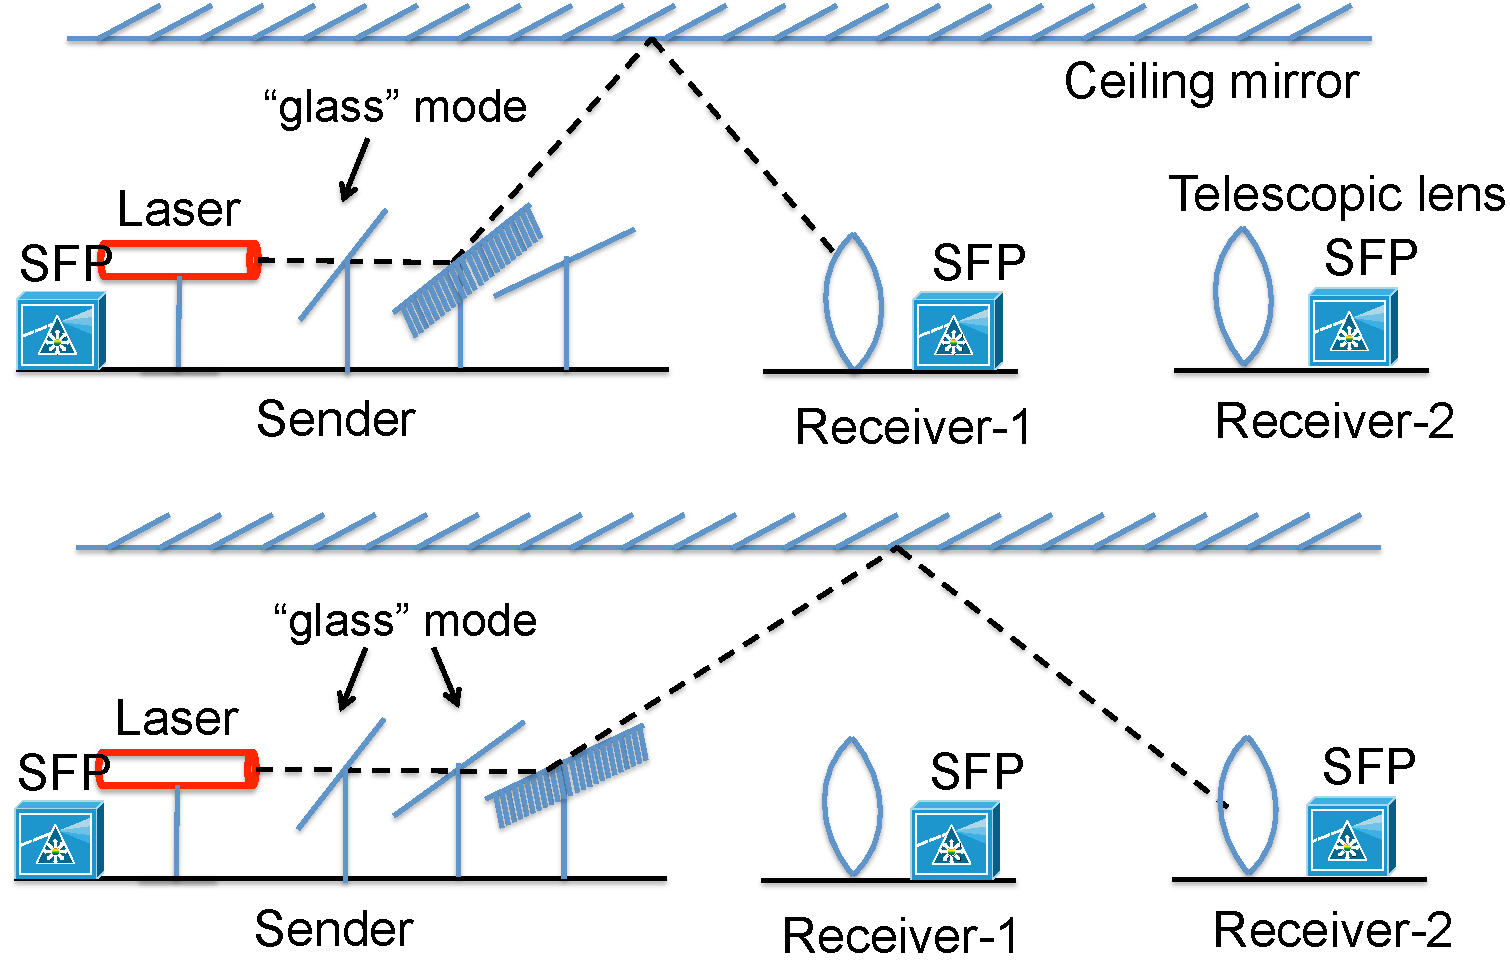
\includegraphics[width=150pt]{Figures/SM-fig.pdf} &
%\hspace{0.5in} &
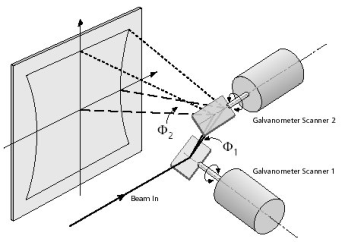
\includegraphics[width=1.5in]{Figures/GM-fig.pdf} \\
(a) Switchable mirror \red{[sd] update fig.}& (b) Galvo mirror\\
\end{tabular}
\caption{ Beam re-direction approaches. (a) A dedicated-alignment beam re-direction approach using SM. (Top) The second SM is in reflection mode, redirecting the beam to Receiver 1.  (Bottom) The second mirror is now transparent and the third mirror is in reflection mode, directing the beam to Receiver 2. (b) Beam steering with GM. Two mirrors direct incident beam into a rectangular cone.}
\vspace{0.05cm}
\label{fig:beam-redirect}
\end{figure}

\paragraph*{Approach I: Beam Switching using Switchable Mirrors}

Here, each beam path is 
\blue{pre-configured statically and remains fixed during normal operation.}  The active beam path is then selected among several candidate beam paths so that links between
a given TX and a chosen subset of RX's can be formed.  One approach to do this is to use switchable mirrors (SMs) made from a special liquid crystal material that can be electrically controlled to rapidly switch between reflection (mirror) and transparent (glass) states in milliseconds time scale~\cite{sm}. 
Referring to Figure~\ref{fig:beam-redirect}(a), each FSO device will be equipped with multiple SMs.  Each SM will be pre-aligned to a dedicated beam path. The desired link is established by placing one of the SMs on the TX in the mirror state and the other SMs in the transparent state. An analogous arrangement will be made at the other end (not shown). At any instant, only a subset of candidate links is active (one per FSO) based on the SMs’ states.  A mirror fastened to the ceiling redirects the beam back to the receiving rack, making efficient use of the above-rack space while minimizing interference. Each SM is oriented appropriately at pre-configuration. This is directed by 
pre-configuration topology design (Section~\ref{sec:topology}). 

The actual machinery for the pre-configuration may consist of
servos that orient SMs and/or the TX/RX to a pre-calculated position and then
the alignment mechanism described before triggers using a feedback from the RX, perhaps scanning
a general area to receive the strongest beam. Note the speed 
of such pre-configuration is not a central issue in our design. 

%\red{A custom, hand-held mechanical adjusting mechanism can be used that will be attached temporarily to SM assembly and adjust each mirror along the calculated orientation.} \vyas{hand-held is weak... maybe have sthg like offline we can compute coordinates etc...} 

\paragraph*{Approach II: Beam Steering using Galvo Mirrors}

In beam steering, the optical system can dynamically re-direct the beam on command and in real time.  This requires computer-controlled movable optics. Among the many possible candidates, one promising approach is to use a galvo mirror (GM) system.  Shown in Figure~\ref{fig:beam-redirect}(b), two computer-controlled, motorized mirrors are mounted at right angles direct incident beam into a rectangular cone.  The (fixed) incident beam can thus be directed into a rectangular cone under computer control.  Commercially available systems~\cite{} 
can provide a cone half angle ($\Phi_1$ and $\Phi_2$) of $\pm 20^\circ$, for a total rectangular cone angle of 
$40^\circ$ in both directions.  A typical pointing accuracy is within 15 $\mu$rad~\cite{}, resulting in a beam positioning precision within 1.5mm for beam paths of up to 100m. GM provides some advantages relative to SM. Since GM can steer on a continuous scale no additional alignment mechanism is necessary as in SM. Also, GM can re-direct the beam to any number of FSOs within the cone in contrast to SMs that provide only a small number of beam paths. \red{The re-direction latencies are however comparable or better in GMs.} However, the limitation of GMs is a limited steering angle that makes the network topology dependent on layout geometry and rack locations. To address this
GMs and/or TX/RX can be oriented appropriately at pre-configuration using
a mechanism described in connection with SMs. 
Also, third servo and mirror combination can be used to increase the angle. Commercially available GMs are also 
generally more expensive than SMs, with cost dependent on precision and speed. Commercially available GMs 
may not have the form factor we desire (as they have a different use case), but a custom design is certainly possible to achieve custom angles and form factors. \red{Exploring such design choices will be part of our study.} 

\blue{We conclude by noting that several other approaches for steering
will be feasible as technology matures. For example, commodity MEMS mirrors~\cite{}
can provide similar functionality as GM, with a higher speed and precision
while taking up much less space. But at this time available mirror sizes are smaller than 
potential beam diameter requirements in \ArchName. Also, more sophisticated
phased array-based approaches have been shown to be feasible~\cite{} and may become
commercially available in the future.} 

%\paragraph*{Integrating Emerging Technologies}
%\blue{The previous design approaches are based on technology available today, to provide a guaranteed path forward. During the project, however, an exhaustive search of emerging and less-known technologies will be conducted to explore additional options in the photonics and optoelectronics communities for beam steering, alignment, and range. Examples include MEMS-based switchable mirrors~\cite{}, low-cost, high range-of-motion servos, low-cost, highperformance aspheric focusing optics (as used in phone cameras), and custom-designed systems built in-house.}


\begin{figure}[t]
\centering
%\vspace{1.5in}
\begin{tabular}{cc}
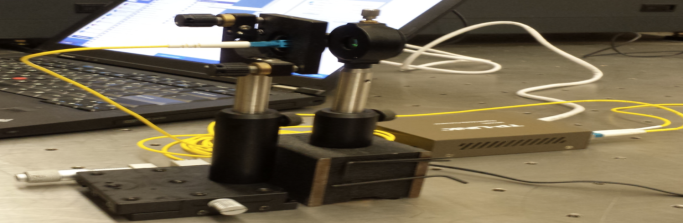
\includegraphics[width=4.5in,height=1.5in]{Figures/optics-layout.pdf} &
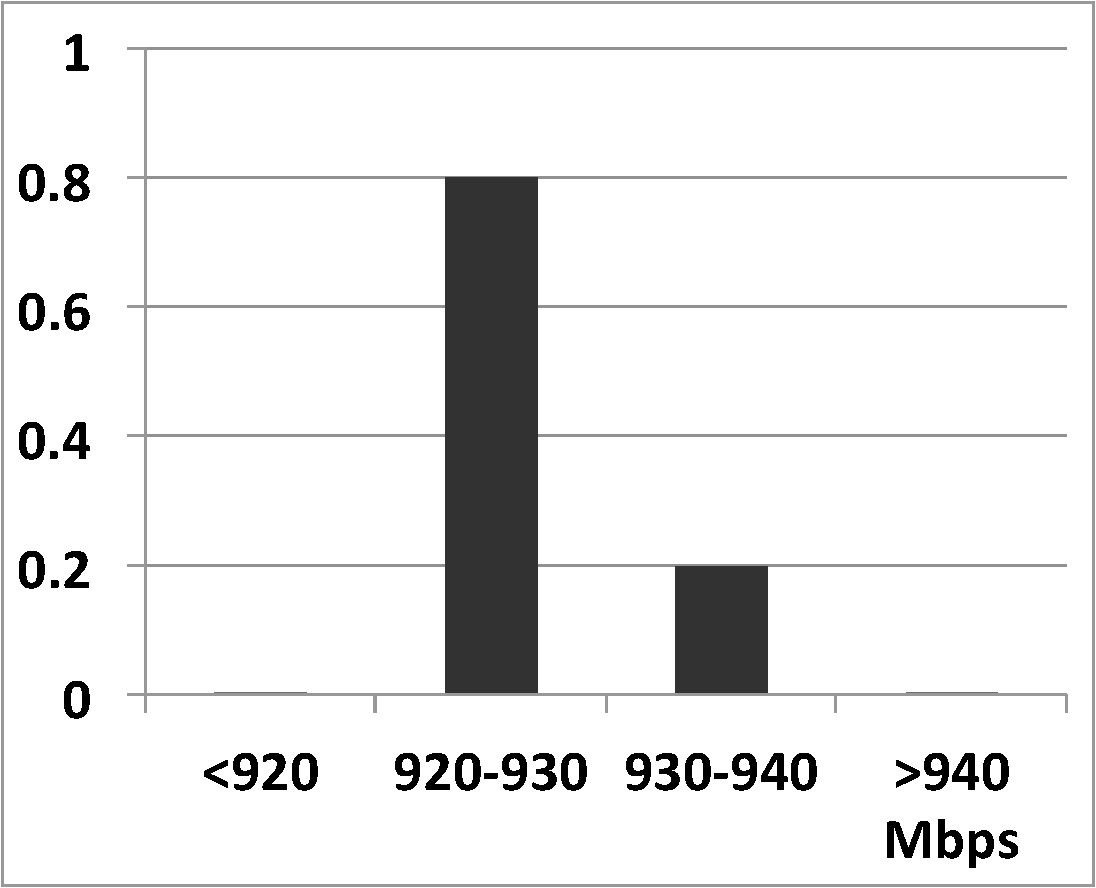
\includegraphics[width=1.8in]{Figures/link-thrpt.pdf} \\
(a) Experimental prototype \red{[sd] placeholder fig.} & (b) Link characterization\\
\end{tabular}
\caption{(a) Experimental prototype showing FSO communication using SFP. (b) Distribution
of per-second TCP throughputs (in Mbps) over a continuous 30 hour period on the FSO link (1Gbps) over 7.5m.}
\label{fig:optics-layout}
\end{figure}


\subsection{Early Demonstration of  Feasibility: Proof-of-Concept Prototype}

We developed a proof-of-concept prototype to demonstrate free space communication using 
commodity optical SFPs. 
See Figure~\ref{fig:optics-layout}. The prototype uses a pair of  1Gbps SFPs using 1310nm laser. Instead of launching the beam directly from the SFP we launch from a single mode optical fiber that is connected to the TX SFP on one end with the other end terminating in free space. Due to the narrow $8-10 \mu\mbox{m}$ fiber diameter the initial beam divergence is very large. An achromatic doublet lens is used to collimate the beam to a roughly 4mm diameter waist with the fiber tip positioned at the focal point of the lens. An optical bench and translating mounts help in the positioning. The collimated beam propagates up to a distance of 7.5m where an identical lens re-focuses beam on the detector of the RX SFP. Since the SFP used here uses two separate optical paths (for duplex operation), the return link is closed using a regular fiber. This way standard network protocols can be run to characterize the free space link. Two laptops are connected to the SFPs via media converters and TCP throughput experiments (with forward direction going over free space) are run for over 30 continuous hours. See the distribution of per sec throughputs in Figure~\ref{fig:optics-layout} that demonstrates an extremely stable link
with performance statistically similar to the ‘wired’ case (both links using fiber). The quality of link is also studied when the TX-RX are misaligned. The TCP throughput is stable up to a transverse shift of $\pm0.7$mm showing a great promise in addressing alignment issues. Beyond this the throughput drops sharply going to zero within another 0.1mm.

We have also built a proof-of-concept prototype to evaluate the viability of switchable mirrors. Here, we have used a 12" x 15" switchable mirror (SM) from Kentoptronics~\cite{sm}
tuned for the IR spectrum; and normal mirrors. The switching latency of the SM is found to be around 250 msec. Because the switching latency is proportional to the SM’s surface area~\cite{sm-size}, we estimate a $<5$ msec latency for a small (1" x 1") SM we propose to use. Finally, we have confirmed that the FSO beam can be reflected from conventional mirrors with no loss in TCP throughputs even after multiple reflections. 


\vyas{just for consistency this might look we havent done prelim work in the
otther sections .. how do we alleviate that fear?}\samir{Fixed by a change in subsection title.
I think this is OK.}

